\section{Techniques Implemented} 
\label{sec:exp}

After explaining the theory of several approaches we now describe our implementations. The proposed algorithm are not always fitting to 
the principle of the games or has a lot of parameter that has to be adjusted to have good results. We first point out same basic strategies
for example staying alive.


\subsection{Stay Alive} 

We implemented two different Stay Alive Agents that has the aim just to act safe and hopefully randomly win the game.
Even if there is the possibility to simulation an action, there is all the time an uncertainty. All objects of the games in our competition
could - but has not - to act randomly. If we are using the \textit{advance} function that allows us to simulate one step that just
one possible state of the future. This implies even if we are not dying at our simulation we could die at the real game.

One approach is to simulate the next action $n$ times. If the agent does not die for this simulations the next action should be safe.
The problem is to set a good value for $n$. If the value is to large not all the possible actions could be tested. Otherwise 
if it's to small the probability that it's even unsafe grows.
From the resulting safe action set there could be randomly choosen the final action.

\begin{figure}
\centering
\begin{minipage}{.5\textwidth}
  \centering
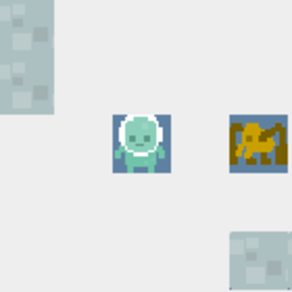
\includegraphics[scale=0.8]{images/safe.pdf}
\caption{Advancing safe actions}
\label{fig:safe}
\end{minipage}%
\begin{minipage}{.5\textwidth}
\centering
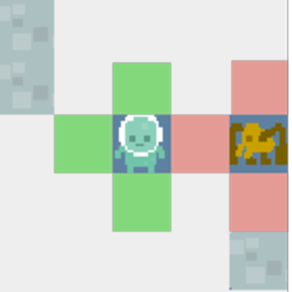
\includegraphics[scale=0.8]{images/safe_grid.pdf}
\caption{Grid search for safe actions}
\label{fig:safe_grid}
\end{minipage}
\end{figure}



Suppose there is a game situation like in~\cref{fig:safe} the action \textit{RIGHT} is definitely unsafe what 
should after an amount of $n$-action be clear.

Another idea is to analyse the grid around the agent. Assume that each enemy could only move one field at the grid
at one game step there is a $5x5$ grid that needs to be analyzed. If an enemy at this grid exists one action is
maybe unsafe. If not the enemy won't die for sure.




At the~\cref{fig:safe_grid} you can see the action that could be excluded without doing any simulation at the game.
The possible next fields (excluded the current position if agent does nothing) are marked green. The possible positions
of the enemy are red. The action RIGHT is by using the grid search unsafe. 
At first glance it looks faster and better to only look at the grid, but there might be some problems for unknown games:

\begin{itemize}
  \item One problem is to classify the game objects at the grid. The grid search is only good if we know that this objects represents an enemy. Otherwise
  we also classify walls as unsafe.
  \item Not every enemy could move to all directions. have a look at the figure 
\end{itemize}



\subsection{Heuristic based} 
 
If the action is only safe the will be the problem that no target is forced because the selection happens randomly.
Therefore a heuristic is used to evaluate one state and get a score. When we previously know the game
that would be one good approach. But whenever the game is unknown the result will be completely different.
One heuristic could be very good for example where the agent could kill an enemy. But if in another game
the enemy will kill us the heuristic let commit us suicide.

To fix that we had two different ideas. On the one hand we could implement a dynamic heuristic that is changing over time
and learn from the environment. On the other hand there could be a third instance that we called \textit{Explorer} 
that is learning from the environment and creating a knowledge-base. 
To use this idea always for further approaches we forced on the second idea.

During the construction time the agent only explores the environment. 
First of all he creates a list with all interesting targets that exists at the level. For all of them he sends pheromones into the grid
and simulate until the agent dies. 
For all the simulation there is a global class the \textit{Simulator} that automatically make inferences from the observations.
The knowledge base is the environment class that contains information to blocking, scoring, winning and loosing game objects (sprites).
This two classes follows the singleton pattern and could be created by using the factory (cf.~\cref{fig:sim_classes}).
Additional information that you can see at the figure is the game detection that is explained later and the field tracker that keeps 
information about all fields at the grid and how often the agent visited each one.

\begin{figure}
\centering
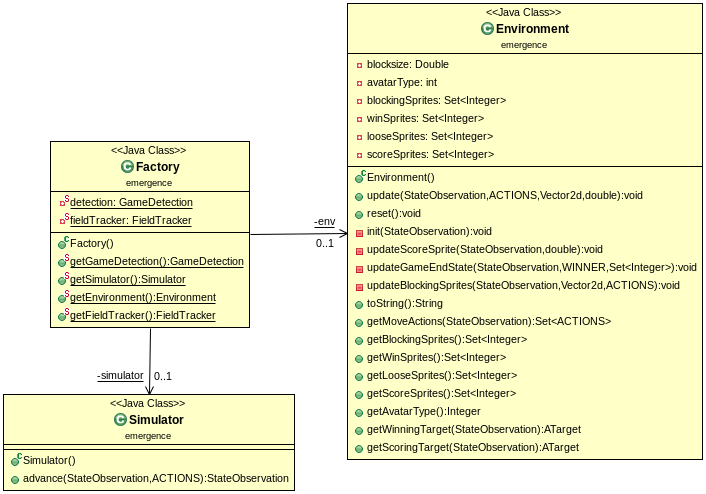
\includegraphics[scale=0.5]{images/classes.png}
\caption{Class diagram of the simulator and environment structure}
\label{fig:sim_classes}
\end{figure}


When the explorer find the winning or scoring objects a heuristic is initialized. We used a heuristic with that 
calculates the distance to one target by using the mannhatten distance. To reach this target we use an astar 
algorithm with three modifications.

Every game step the astar algorithm is executed from scratch even if we found the target in the last iteration.
We use an safety approach for the first action to ensure the next action we maybe choose is safe. For that we
use the principle of the stay alive agent. The astar algorithm needs to hold all the states in memory.
This leads to a very fast growing open list with a lot of states. We introduce a \textit{maxStates} variable. 
Whenever the open list of the astar algorithm is larger than this variable the list is cut in a half.
Additionally we use for our simulations the simulator and use the knowledge base. Normally all children of
a state are added to the open list. We only add all the children to the list of that we assume we will get a 
new position. Since we know from the Environment class which objects are blocking, we could use that information
for a smarter iteration.


\subsection{MCTS Tree} 

The theory of MCTS-treesearch is described in section 3. The standard approach was modified to fit our problem. The whole MCTS algorithm is computed in the class \textit{MCTSStrategy} which is used by the \textit{MCTSAgent} and the \textit{MCTSHeuristicAgent}.

\subsubsection{tree policy}
Our tree policy iterates trough the tree, starting at the root node. When a node is not fully expanded, a randomly chosen children node is generated. We tried out some other ways to chose the children, but random selection worked best. If we reach a fully expanded node the tree policy uses a modified UCT formula

\begin{equation}
 	UCT = \frac{c.Q}{c.V + ep * r} + \sqrt{\frac{\ln (n.V+1)}{c.V}}
\end{equation} 

to chose the children node. Where \textit{n} is the node and \textit{c} the actual children. \textit{Q} is the reward of a node and \textit{V} the number of visits, more precise the number of times the tree policy had chosen this node. The exploitation term is computetd by dividing the reward of the child by the number of vistis and a random factor to avoid divisions by zero. This term is big for nodes whose reward is high on average.
When the childs number of visits are small in comparison to the others, the second term (exploration) will be big. We tried out some other varaints and factors but this solution has the best results. It is very close to the original UCT formua (see section 3).   

\subsubsection{default policy \& backpropagation}

The default policy tries to figure out how good the given node from the tree policy is. To do that, a simulation with the correspond state observation and random actions is done. It is repeated until the hypotethical level of the simulated node reaches the before defined maximum (maximal depth of the tree). At the beginning, when the tree is small, more simulations are executed. Later, when we have already grown our tree, only a few simulations are executed. We chose this approach because at the begnning we have no information about the node and its neighbourhood so we have to compute more simulations....
When the simuation is finished a reward is generated from the last state observation by the delta heuristic which is descibed later. The win, loss and score were considered.
The backpropagation iterates from the node which was expanded by the tree policy to the root, guided by the father references of every node. To every visited node the reward is added and weigthed with a before specified value.

\subsubsection{rolling horizon}

The implementation of a rolling horion working on it......

\begin{itemize}
  \item tree policy
  \item default policy
  \item act choosig -> most visited node
\end{itemize}
























\subsection{Evolutionary algorithm} 

The theory of the evolution has to be mapped to the gaming problem. Each candidate of our population is
a list of actions that could be executed. To evaluate the fitness of a candidate we are using the
simulation function that is provided by the game. 
The score

\begin{equation}
s = \sum_{t=0}^n (H(s_t) - H(s_{t-1}))
\end{equation}

is calculated by using the function

\begin{equation}
    H(s_i, s_{i-1}) = 
\begin{dcases}
    10, & \text{if isWinner}  \\
    -10, & \text{if isLooser}  \\
    score(s_i) - score(s_{i-1}), & \text{otherwise.}
\end{dcases}
\end{equation}

what we called delta heuristic function.

We implemented two very naive operations on the pool. The crossover is done by
select for 50 \% the action of the first or the second individual (cf.~\cref{fig:crossover}).

\begin{figure}[H]
\centering
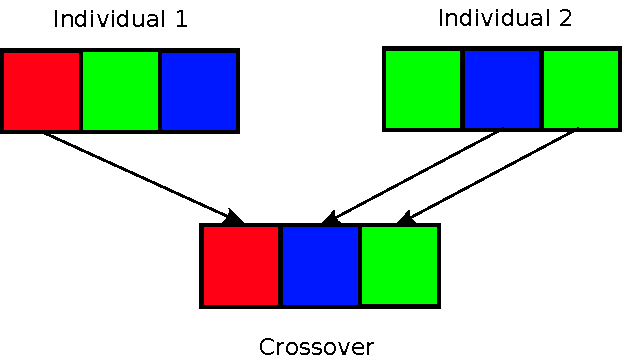
\includegraphics[scale=0.6]{images/crossover.pdf}
\caption{Crossover of an individual}
\label{fig:crossover}
\end{figure}

The mutation is implemented by doing an crossover with an random individual.
We fixed for all evaluations runs the mutation probability to $0.7$ which implies a crossover 
probability of $0.3$.

We had several problems with the limited time for the evolution.
For that we want to have always a good starting pool and use our information from the last
game step. All candidates from the last final pool of the last game step are used for the initialization.


\begin{figure}[H]
\centering
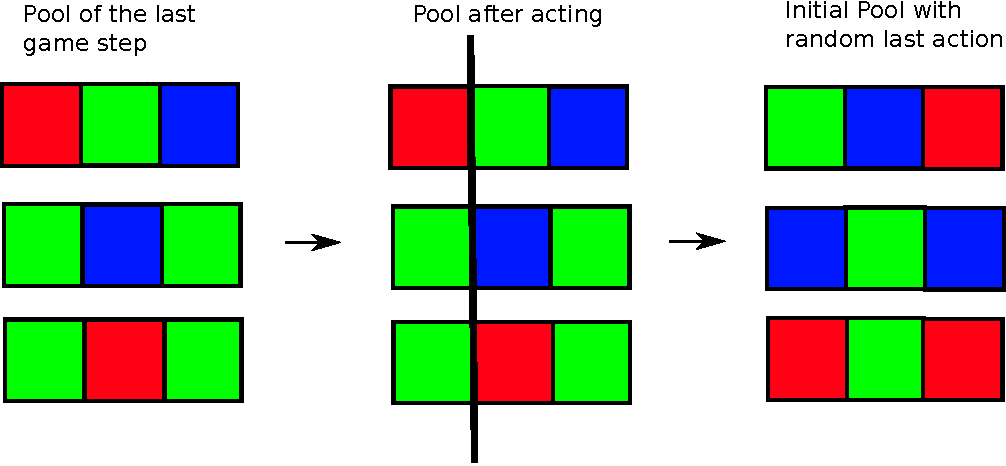
\includegraphics[scale=0.6]{images/sliding_window.pdf}
\caption{Sliding Window}
\label{fig:sliding_window}
\end{figure}

For that we use the principle of a sliding window (cf.~\cref{fig:sliding_window}). The first
action from the last pool is removed because the agent was acting like this at the last game step. Then
to keep the action length fix there is added one random action to the action path.
By using that principle we are not throwing our last simulations away.

There is also the problem that for different games the simulation time differs. If we have many game objects that 
need to be updated and checked for collision, the simulation time increases.
But to find a good value for the pool size we need to know the calculation time.
As a fix for this we introduced the adaptive path length that reduces or increases the actions
of every individual.
For that we forced to get always the fourth generation. On the one hand if we stay for example at the initial
pool because the evaluation takes to long we will reduce the path length. On the other hand if the agents acts like 
the seventh generation we force to have a long time planing by increasing the path length.

Another problem that we tried to fix is to avoid situations where no individual has a positive score or many has a score of zero. That means each 
candidate is not gaining points. Our first implementations solved such a tie randomly. 
The randomness could be disabled by using a heuristic. If we would always use the same heuristic that would not work
for all the games because they have different aims. 
So we used a heuristic switch after $n$ time steps to have also a long time planing strategy.


  
  
\subsection{Game Detection} 
  
Another technique we have implemented is a detection of a known game. We know the 10 games from the test-set and the 10 games from the validation-set, the 10 test-set games are unknown. The Goal of the Gamedetection is to improve the score and the number of wins in the two known game-sets without decreasing the score and the number of wins in the unknown test-set. To do that, the standard parameters of the Algorithm are used when no game is detected, otherwise the optimal parameters for this game are used. These parameters we figured out for some difficult games in which the standard parameters give bad results. To detect a game we generate a String of all Objects (npc, movable, immovable, ect...) and store the Hash value of this String. All the hashes from the known games are stored, in a running Game we generate another String of these Objects and compare the generated hash value to the stored ones. 